%%=============================================================================
%% Conclusie
%%=============================================================================

\chapter{Conclusie}
\label{ch:conclusie}

% TODO: Trek een duidelijke conclusie, in de vorm van een antwoord op de
% onderzoeksvra(a)g(en). Wat was jouw bijdrage aan het onderzoeksdomein en
% hoe biedt dit meerwaarde aan het vakgebied/doelgroep? 
% Reflecteer kritisch over het resultaat. In Engelse teksten wordt deze sectie
% ``Discussion'' genoemd. Had je deze uitkomst verwacht? Zijn er zaken die nog
% niet duidelijk zijn?
% Heeft het onderzoek geleid tot nieuwe vragen die uitnodigen tot verder 
%onderzoek?

\section{GDPR}
\label{sec: Conclusie GDPR}

Rekeninghoudend met de informatie die verkregen werd bij de literatuurstudie, kan er een antwoord geleverd worden op de onderzoeksvraag.

Indien de regels van de GDPR nageleefd worden inzake het verwerken van informatie van personen, kan er een systeem opgezet worden dat volgzaam is aan de wetgeving, en toch in staat is gepersonaliseerde zoekopdrachten uit te voeren. 

Er zal een eenduidig en ondubbelzinnig beleid moeten worden opgesteld dat de gebruiker al dan niet kan accepteren.
 Indien de gebruiker niet akkoord gaat met het beleid, of zijn informatie slechts deels ter beschikking wenst te stellen, zal hierbij rekening gehouden moeten worden dat de resultaten van zoekopdrachten in sommige gevallen minder of zelfs niet gepersonaliseerd kunnen worden.

De keuze moet hierbij volledig in handen van de gebruiker liggen, en deze moet via het beleid op de hoogte gesteld worden van de doeleinden waarvoor zijn informatie gebruikt zal worden, om zo een beslissing te maken. In de voorgestelde toepassing zal dus duidelijk vermeld moeten staan dat zijn persoonlijke informatie enkel en alleen gebruikt wordt voor het aanbieden van gepersonaliseerde zoekresultaten.

Bij het aanmaken van een account zal nogmaals een beleid moeten opgesteld worden, waarin duidelijk vermeld staat waarvoor de data die ingevuld wordt bij de creatie van het account gebruikt zal worden. In deze toepassing zal het dus gaan over de gegevens over de woonplaats van een gebruiker, leeftijdscategorie, naam, etc.

Bijvoorbeeld voor het gebruik van de data over de woonplaats zal dus duidelijk verwoord moeten worden dat deze data gebruikt wordt voor het linken van personen binnen één gezin.

Ook zal er geen data mogen bijgehouden worden die niet relevant is voor de doelstellingen, gegevens zoals bijvoorbeeld een telefoonnummer zijn niet van belang voor onze doelstellingen, en mogen dus niet verwerkt worden. De gebruiker moet steeds in staat zijn om zijn gegevens op te vragen of deze te laten wissen, en dit moet steeds zonder onredelijke vertraging gebeuren.

Hiermee is de onderzoeksvraag beantwoordt; ja, het is mogelijk om een systeem op te stellen met een gepersonaliseerde zoekfunctie die als legaal wordt aanzien onder de wetgeving omtrent GDPR.

\section{ ElasticSearch}
\label{sec:Conclusie Elasticsearch}

Elasticsearch is zeer snel en eenvoudig in het gebruik als het gaat over het vinden van producten die relateren aan de gebruiker zelf. Uit het onderzoek bleek ook dat specifieke zoektermen en filters relatief eenvoudig te implementeren zijn.

Het rekening houden met andere variabelen van een persoon zoals geslacht, leeftijdscategorie, etc. zijn wel mogelijk bij het genereren van aanbevelingen bij een zoekopdracht. Dit kan door middel van gebruikers te vergelijken op basis van bijvoorbeeld hun gemeenschappelijke zoekopdrachten.

Elasticsearch biedt ook de mogelijkheden om een graaf met de relaties tussen de verschillende documenten op te slaan, maar deze is niet zomaar verkrijgbaar, hier is een Platinum of Enterprise licentie voor vereist. Het is mogelijk om op deze manier dan toch rekening te kunnen houden met familiale relaties, alsook filters toe te passen op de zoekopdrachten.

\section{ Neo4j}
\label{sec:Conclusie Neo4j}

Neo4j, als graph databank, staat toe om gebruik te maken van alle relaties tussen de verschillende producten (nodes) om aanbevelingen te genereren. Ook zijn er enkele algoritmen reeds ingebouwd in een Graph Data Analysis plugin, die zorgen voor de meest performante werkwijze.

Qua eenvoud van implementatie is Neo4j de betere keuze, mede met dank aan het feit dat alles visueel kan toegelicht worden door simpelweg naar de graaf te kijken. 

Zowel het gebruik van de graaf, als het zoeken op basis van een tekstveld zijn mogelijk in Neo4j zonder dat hier extra kosten aan vasthangen voor licenties. 

\section{Resultaat}
\label{sec:Resultaat}

Er kan dus geconcludeerd worden dat elk van deze technieken uitblinkt in zijn eigen branche. De resultaten worden nog eens opgesomd in volgende tabel, waar al snel duidelijk wordt dat ze zeer sterk tegen elkaar opwegen. Toch is het zo dat de ene technologie de andere niet kan vervangen op gebied van performantie en eenvoud.

\begin{table}[hbt!]
	\begin{tabular}{l|l|l|}
		\cline{2-3}
		& \cellcolor[HTML]{C0C0C0}Neo4j & \cellcolor[HTML]{C0C0C0}Elasticsearch \\ \hline
		\multicolumn{1}{|l|}{\cellcolor[HTML]{EFEFEF}Gebruiksgemak (subjectief)}      & 8/10                          & 7/10                                  \\ \hline
		\multicolumn{1}{|l|}{\cellcolor[HTML]{EFEFEF}Simpel zoeken}                   & Ja                            & Ja                                    \\ \hline
		\multicolumn{1}{|l|}{\cellcolor[HTML]{EFEFEF}Geavanceerd zoeken}              & Ja, niet zo performant        & Ja                                    \\ \hline
		\multicolumn{1}{|l|}{\cellcolor[HTML]{EFEFEF}Relaties tussen producten ontdekken}              & Ja, meerdere algoritmen       & Nee                    \\ \hline
		\multicolumn{1}{|l|}{\cellcolor[HTML]{EFEFEF}Persoonsgegevens gebruiken}              & Ja    & Ja                    \\ \hline
		\multicolumn{1}{|l|}{\cellcolor[HTML]{EFEFEF}Familierelaties gebruiken}       & Ja, eenvoudig \& snel         & Nee          \\ \hline
		\multicolumn{1}{|l|}{\cellcolor[HTML]{EFEFEF}Gebruik maken van productkennis} & Ja                            & Ja, maar licentie nodig               \\ \hline
	\end{tabular}
	\caption{\label{tab: Bevindingen Neo4j & Elasticsearch} Bevindingen Neo4j \& Elasticsearch}
\end{table}




Het doel van dit onderzoek was om te achterhalen of een van deze technologieën een oplossing biedt voor het implementeren van gepersonaliseerde zoekopdrachten in e-commerce toepassingen. In dit hoofdstuk worden de onderzoeksvragen concreet beantwoord op basis van het onderzoek en de conclusies, en worden deze kort toegelicht.


Het opstellen van dergelijk systeem wordt als legaal aanzien onder de wetgeving rond GDPR, indien er aan de voorwaarden wordt voldaan zoals besproken in hoofdstuk 4.1, hiermee wordt de eerste onderzoeksvraag beantwoordt.
	
Beide technologieën bieden een mogelijkheid om een gepersonaliseerd zoeksysteem uit te werken. Neo4j kan dit zonder problemen  door gebruik te maken van enkel de relaties en nodes, en een query met een tekstveld naar de databank te sturen.
In ElasticSearch kunnen we gebruik maken van enkele meer geavanceerde filters, maar zijn we beperkt tot de informatie die we over de gebruiker hebben. Deze informatie omvat bijvoorbeeld leeftijd, geslacht, etc. of voorkeuren die deze gebruiker zelf heeft ingesteld. Dit biedt een antwoord op de tweede onderzoeksvraag.
	
Om een antwoord te geven op de derde onderzoeksvraag, kan er uit de vorige paragraaf afgeleid worden dat beide technologieën de mogelijkheid verschaffen om productdata te combineren met persoonlijke data zoals geslacht, leeftijd, provincie, etc. 

Uit het onderzoek bleek dat Elasticsearch als basis niet geschikt is voor het leggen van connecties tussen personen, en dus ook niet voor het leggen van connecties tussen producten. Indien men een licentie aankoopt kan er wel gebruikt gemaakt worden van Graph functionaliteiten. Hiermee wordt de laatste onderzoeksvraag beantwoord.


\subsection{Conclusie}
\label{subsec:finalConclusie}

In de context van een bedrijf die met behulp van één van deze twee technologieën een gepersonaliseerd zoeksysteem wil uitwerken, is ElasticSearch de beste optie. Een bedrijf zal gebruik maken van een Enterprise licentie, waar de Graph API functionaliteit beschikbaar is.

Elasticsearch biedt dus alle functionaliteit van Neo4j in de vorm van een Graph databank, met daar bovenop nog eens de mogelijkheid om complexe zoekopdrachten met verscheidene filters zeer snel te verwerken. 

Elastic geeft ook duidelijk aan hoe snel er support verwacht kan worden afhankelijk van de licentie. Voor Enterprise gebruikers is dit bijvoorbeeld één uur voor zeer dringende zaken. 
Een compleet overzicht hiervan is te vinden in Figuur \ref{fig:elasticSupport}

\begin{figure} [ht]
	\centering
	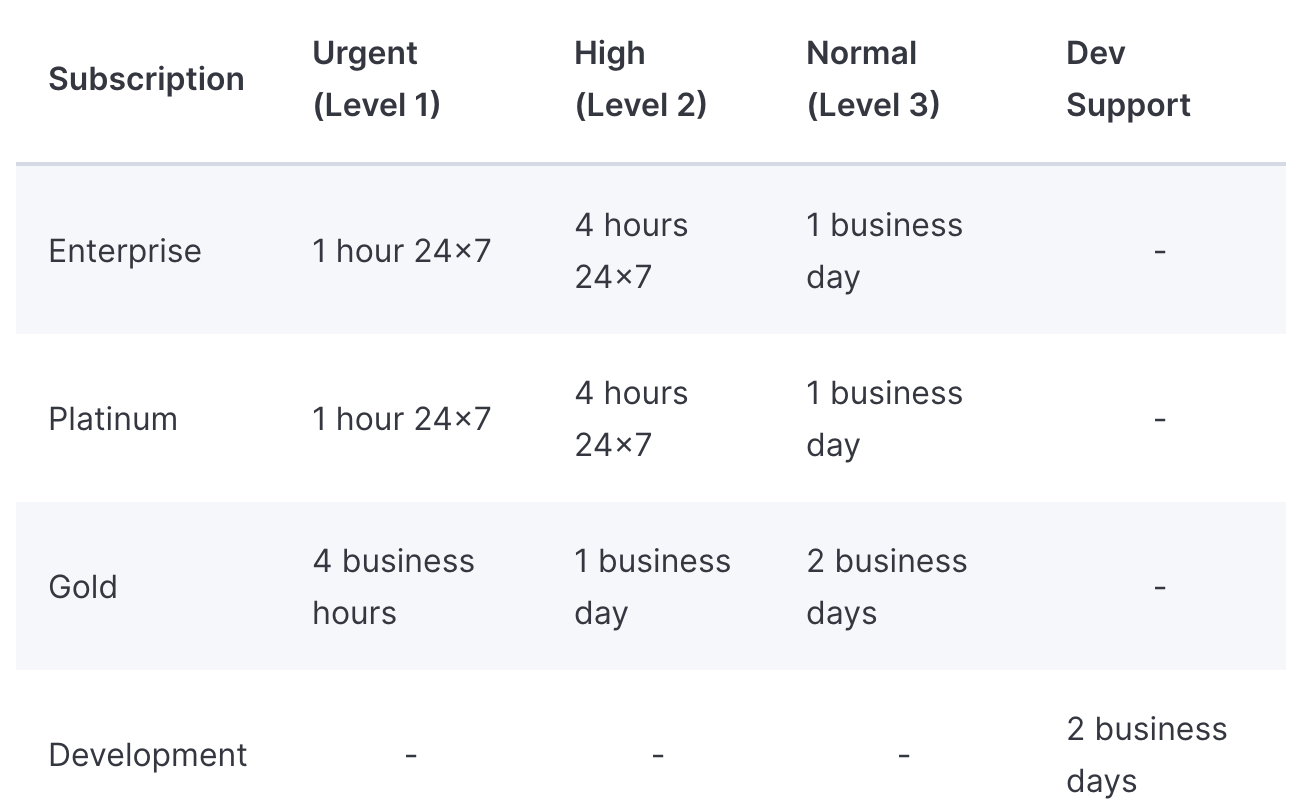
\includegraphics[width=0.95\textwidth]{img/elastic-support}
	\caption{Elastic.co Support}
	\floatfoot{Source: elastic.co/support/welcome}
	\label{fig:elasticSupport}
\end{figure}



\subsection{Alternatief}
De literatuurstudie wees ook uit dat een Knowledge Graph gebruikt kan worden om aanvullende informatie te verschaffen bij het genereren van gepersonaliseerde zoekresultaten. 

Een alternatieve optie is dus om beide platformen te combineren, en elkaar te laten aanvullen. Een voorbeeld hier van is om de resultaten van een zoekalgoritme in Neo4 te combineren met de scores die gevonden werden in Elasticsearch. 

Deze ontdekking zet de weg open naar verder onderzoek in hoe deze twee platformen efficiënt samen gebruikt kunnen worden, en hoe de modellen die in dit onderzoek werden opgebouwd, verder gespecialiseerd kunnen worden om deze combinatie mogelijk te maken. 
